% SPDX-License-Identifier: BSD-2-Clause
%
% Copyright (C) 2026 embedded brains GmbH & Co. KG
%
% Redistribution and use in source and binary forms, with or without
% modification, are permitted provided that the following conditions
% are met:
% 1. Redistributions of source code must retain the above copyright
%    notice, this list of conditions and the following disclaimer.
% 2. Redistributions in binary form must reproduce the above copyright
%    notice, this list of conditions and the following disclaimer in the
%    documentation and/or other materials provided with the distribution.
%
% THIS SOFTWARE IS PROVIDED BY THE COPYRIGHT HOLDERS AND CONTRIBUTORS "AS IS"
% AND ANY EXPRESS OR IMPLIED WARRANTIES, INCLUDING, BUT NOT LIMITED TO, THE
% IMPLIED WARRANTIES OF MERCHANTABILITY AND FITNESS FOR A PARTICULAR PURPOSE
% ARE DISCLAIMED. IN NO EVENT SHALL THE COPYRIGHT OWNER OR CONTRIBUTORS BE
% LIABLE FOR ANY DIRECT, INDIRECT, INCIDENTAL, SPECIAL, EXEMPLARY, OR
% CONSEQUENTIAL DAMAGES (INCLUDING, BUT NOT LIMITED TO, PROCUREMENT OF
% SUBSTITUTE GOODS OR SERVICES; LOSS OF USE, DATA, OR PROFITS; OR BUSINESS
% INTERRUPTION) HOWEVER CAUSED AND ON ANY THEORY OF LIABILITY, WHETHER IN
% CONTRACT, STRICT LIABILITY, OR TORT (INCLUDING NEGLIGENCE OR OTHERWISE)
% ARISING IN ANY WAY OUT OF THE USE OF THIS SOFTWARE, EVEN IF ADVISED OF THE
% POSSIBILITY OF SUCH DAMAGE.

\documentclass[tikz,border=4pt]{standalone}
\usepackage[T1]{fontenc}
\usepackage[scaled]{helvet}
\renewcommand{\familydefault}{\sfdefault}
\usetikzlibrary{arrows.meta,positioning,fit,backgrounds,shapes.geometric}
\definecolor{ebblue}{HTML}{1F4E79}
\definecolor{boxfill}{HTML}{EAF1F8}
\definecolor{codefill}{HTML}{FFF4E0}
\definecolor{codeline}{HTML}{9C6500}
\definecolor{groupfill}{HTML}{F5F5F5}
\definecolor{flow}{HTML}{404040}
\newcommand{\code}[1]{{\ttfamily\scriptsize #1}}
\begin{document}
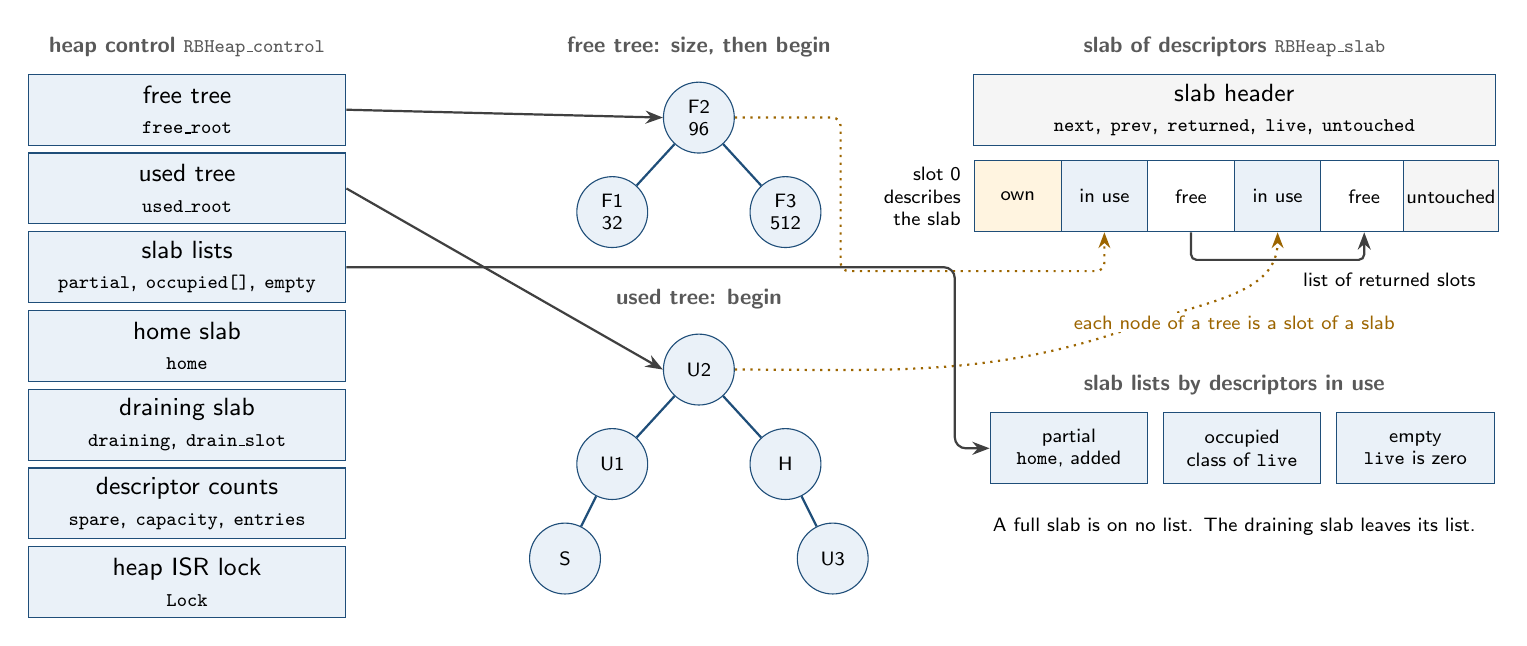
\begin{tikzpicture}[
    font=\small,
    field/.style={draw=ebblue, fill=boxfill, minimum width=40mm,
      minimum height=9mm, align=center, text width=38mm},
    tnode/.style={draw=ebblue, fill=boxfill, circle, minimum size=9mm,
      inner sep=0pt, font=\scriptsize, align=center},
    slot/.style={draw=ebblue, minimum width=11mm, minimum height=9mm,
      align=center, font=\scriptsize, inner sep=1pt},
    link/.style={-{Stealth[length=2.2mm]}, thick, draw=flow},
    lives/.style={-{Stealth[length=2mm]}, dotted, thick, draw=codeline},
    smp/.style={dashed},
    lbl/.style={font=\scriptsize, align=center, fill=white, inner sep=1pt},
    title/.style={font=\footnotesize\bfseries, text=gray!70!black}]
  % Heap control
  \node[title] at (0,8.1) {heap control \code{RBHeap\_control}};
  \node[field] (free) at (0,7.3) {free tree\\\code{free\_root}};
  \node[field] (used) at (0,6.3) {used tree\\\code{used\_root}};
  \node[field] (lists) at (0,5.3) {slab lists\\\code{partial}, \code{occupied[]}, \code{empty}};
  \node[field] (home) at (0,4.3) {home slab\\\code{home}};
  \node[field] (drain) at (0,3.3) {draining slab\\\code{draining}, \code{drain\_slot}};
  \node[field] (count) at (0,2.3) {descriptor counts\\\code{spare}, \code{capacity}, \code{entries}};
  \node[field] (lock) at (0,1.3) {heap ISR lock\\\code{Lock}};
  % Free tree
  \node[title] at (6.5,8.1) {free tree: size, then begin};
  \node[tnode] (f1) at (6.5,7.2) {F2\\96};
  \node[tnode] (f2) at (5.4,6.0) {F1\\32};
  \node[tnode] (f3) at (7.6,6.0) {F3\\512};
  \draw[thick, draw=ebblue] (f1) -- (f2);
  \draw[thick, draw=ebblue] (f1) -- (f3);
  % Used tree
  \node[title] at (6.5,4.9) {used tree: begin};
  \node[tnode] (u1) at (6.5,4.0) {U2};
  \node[tnode] (u2) at (5.4,2.8) {U1};
  \node[tnode] (u3) at (7.6,2.8) {H};
  \node[tnode] (u4) at (4.8,1.6) {S};
  \node[tnode] (u5) at (8.2,1.6) {U3};
  \draw[thick, draw=ebblue] (u1) -- (u2);
  \draw[thick, draw=ebblue] (u1) -- (u3);
  \draw[thick, draw=ebblue] (u2) -- (u4);
  \draw[thick, draw=ebblue] (u3) -- (u5);
  \draw[link] (free.east) -- (f1.west);
  \draw[link] (used.east) -- (u1.west);
  % A slab of descriptors
  \node[title] at (13.3,8.1) {slab of descriptors \code{RBHeap\_slab}};
  \node[draw=ebblue, fill=groupfill, minimum width=66mm, minimum height=9mm,
    align=center, text width=64mm] (shdr) at (13.3,7.3)
    {slab header\\\code{next}, \code{prev}, \code{returned}, \code{live}, \code{untouched}};
  \foreach \i/\t/\f in {0/own/codefill, 1/in use/boxfill, 2/free/white,
      3/in use/boxfill, 4/free/white, 5/untouched/groupfill} {
    \node[slot, fill=\f] (s\i) at (10.55+\i*1.1,6.2) {\t};
  }
  \draw[link, rounded corners=2pt] (s2.south) -- ++(0,-0.35) -| (s4.south);
  \node[font=\scriptsize, anchor=north west] at (14.05,5.35) {list of returned slots};
  \node[font=\scriptsize, anchor=east, align=right] at (9.95,6.2) {slot 0\\describes\\the slab};
  \draw[lives, rounded corners=3pt] (f1.east) -- (8.3,7.2) |- (11.65,5.25) -- (s1.south);
  \draw[lives] (u1.east) to[out=0, in=200] (12.2,4.6) to[out=20, in=270] (s3.south);
  \node[lbl, text=codeline] at (13.3,4.6) {each node of a tree is a slot of a slab};
  % Slab lists
  \node[title] at (13.3,3.8) {slab lists by descriptors in use};
  \node[slot, minimum width=20mm, fill=boxfill] (pl) at (11.2,3.0) {partial\\\code{home}, added};
  \node[slot, minimum width=20mm, fill=boxfill] (ol) at (13.4,3.0) {occupied\\class of \code{live}};
  \node[slot, minimum width=20mm, fill=boxfill] (el) at (15.6,3.0) {empty\\\code{live} is zero};
  \draw[link, rounded corners=4pt] (lists.east) -- (9.75,5.3) |- (pl.west);
  \node[font=\scriptsize, align=center, text width=64mm] at (13.3,2.0)
    {A full slab is on no list.  The draining slab leaves its list.};
  % Processor blocks
\end{tikzpicture}
\end{document}
